\section{Project Details}

\subsection{Ethernet Frame Generation Process}

This section outlines the process of generating Ethernet frames. The generation of Ethernet frames necessitates the configuration of the physical layer transceiver circuitry (PHY) and the development of a controller module. The PHY plays a pivotal role as it connects the Ethernet Media Access Control (MAC) to the physical transmission medium, handling the fundamental Layer 1 functions of the Ethernet protocol. Refer to Figure  \ref{fig:eth-mod-arch} for the detailed architecture of this module.


\subsubsection{Ethernet PHY Configuration}

The Ethernet frame generation is centered around the configuration of the SMSC 10/100 Ethernet PHY integrated on the Nexys4 DDR board, which interfaces with an RJ-45 jack featuring integrated magnetics. A pivotal aspect of this setup is the Reduced Media Independent Interface (RMII) configuration, where the data bus width is set to 2 for transmitting and receiving Ethernet frames. A First-In-First-Out (FIFO) buffer manages the efficient flow of packet data from the source (AXI stream) to the packet generator.
\begin{figure}
    \centering
    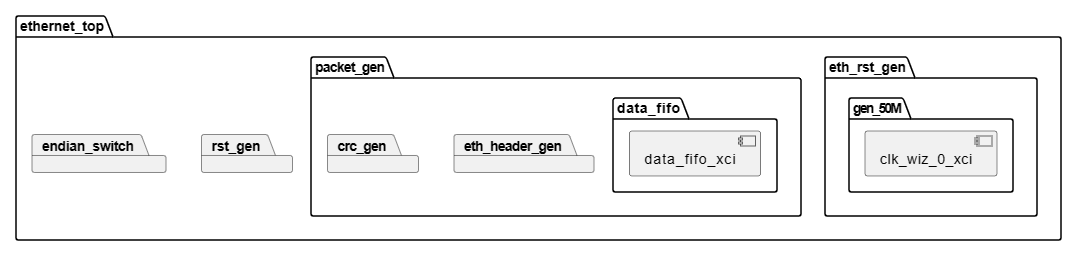
\includegraphics[width=1\linewidth]{Sections//IMPLEMENTATION//images/ModuleETH.png}
    \caption{Ethernet module architecture}
    \label{fig:eth-mod-arch}
\end{figure}
The configuration of the PHY was methodically executed with the following key steps:

\begin{itemize}
    \item Activation of Reduced Media Independent Interface (RMII) mode to improve the efficiency of Ethernet connectivity.
    \item Implementation of auto-negotiation to facilitate support for various operational modes, allowing speeds up to 100 Mbps.
    \item Assignment of the address 00001 to the PHY, enabling unique network identification.
    \item Calibration of each clock signal to counteract skew issues, with the external PHY clock receiving a 45-degree phase shift in comparison to the Reference Clock (Ref\_Clk), ensuring synchronization and reliability.
\end{itemize}





\subsubsection{Controller Architecture and State Machine}

The controller is constructed around a state machine responsible for generating the 802.3 Ethernet packet and frame structure. Refer to Figure \ref{fig:eth-fsm} for the state machine diagram. It encompasses several states and transitions detailed as follows:
\begin{figure}
    \centering
    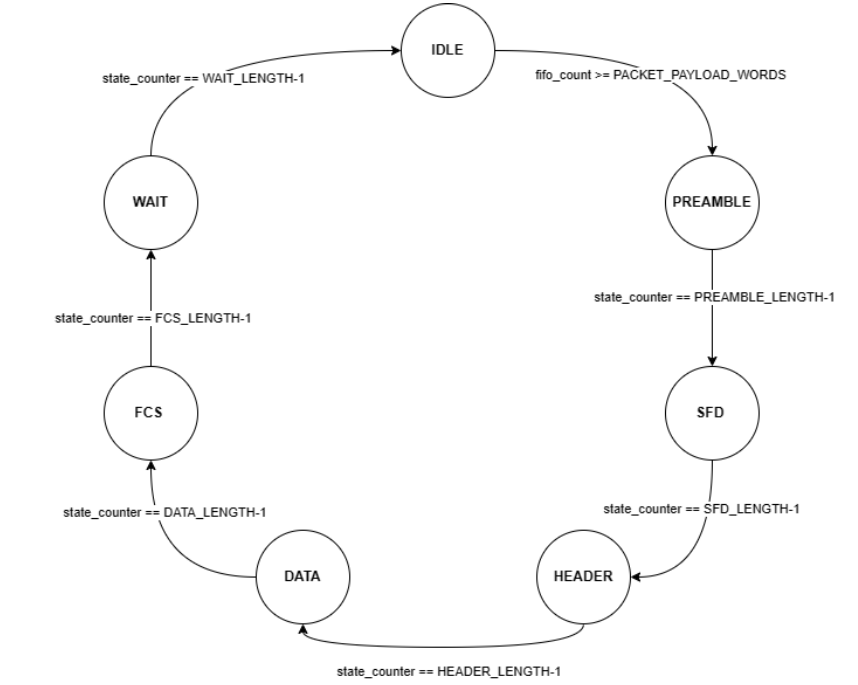
\includegraphics[width=0.75\linewidth]{Sections//IMPLEMENTATION//images/fsm_packet_gen.png}
    \caption{Ethernet packet generator FSM}
    \label{fig:eth-fsm}
\end{figure}
\begin{description}
    \item[IDLE State:] The default state where the system idles until it is prepared to commence frame processing.
    \item[PREAMBLE State:] Upon leaving the IDLE state, the system generates the Ethernet frame preamble in the PREAMBLE state, a sequence critical for synchronization.
    \item[SFD State:] The Start Frame Delimiter (SFD) state succeeds the PREAMBLE state, marking the beginning of the Ethernet frame.
    \item[HEADER State:] After the SFD, the HEADER state is engaged to process the frame's HEADER, which encapsulates vital control and addressing information, including source and destination MAC addresses.
    \item[DATA/PAYLOAD State:] The DATA state involves processing the frame's payload -- the core message conveyed across the network. For initial testing, this payload comprised 32-bit integers generated by an up-counter, facilitating debugging via the Wireshark tool.
    \item[FCS State:] Following the DATA state, the Frame Check Sequence (FCS) state computes a checksum using a linear feedback shift register, applying the standard CRC Ethernet function to verify data integrity.
    \item[WAIT State:] The FCS state is succeeded by the WAIT state, which readies the system either to revert to IDLE or to handle a new frame. This state is instrumental in timing management and prevents premature re-entry to the IDLE state.
\end{description}

Additionally, the controller architecture includes a reset feature and an endianness switch, enabling conformity with various networking protocols.



\subsection{PDM Microphone Audio Capture Process}

The FPGA board is equipped with an ADMP421 chip, which is a Micro-Electro-Mechanical Systems (MEMS) microphone (refer to Figure \ref{fig:pdm-mod-arch} for the implementation overview). The microphone captures audio signals and digitizes them using Pulse Density Modulation (PDM). This process involves a Delta-sigma modulation circuit integrated within the FPGA. PDM is a technique for representing analog signals with a binary sequence, where the density of the pulses correlates with the signal's amplitude.

\begin{figure}
    \centering
    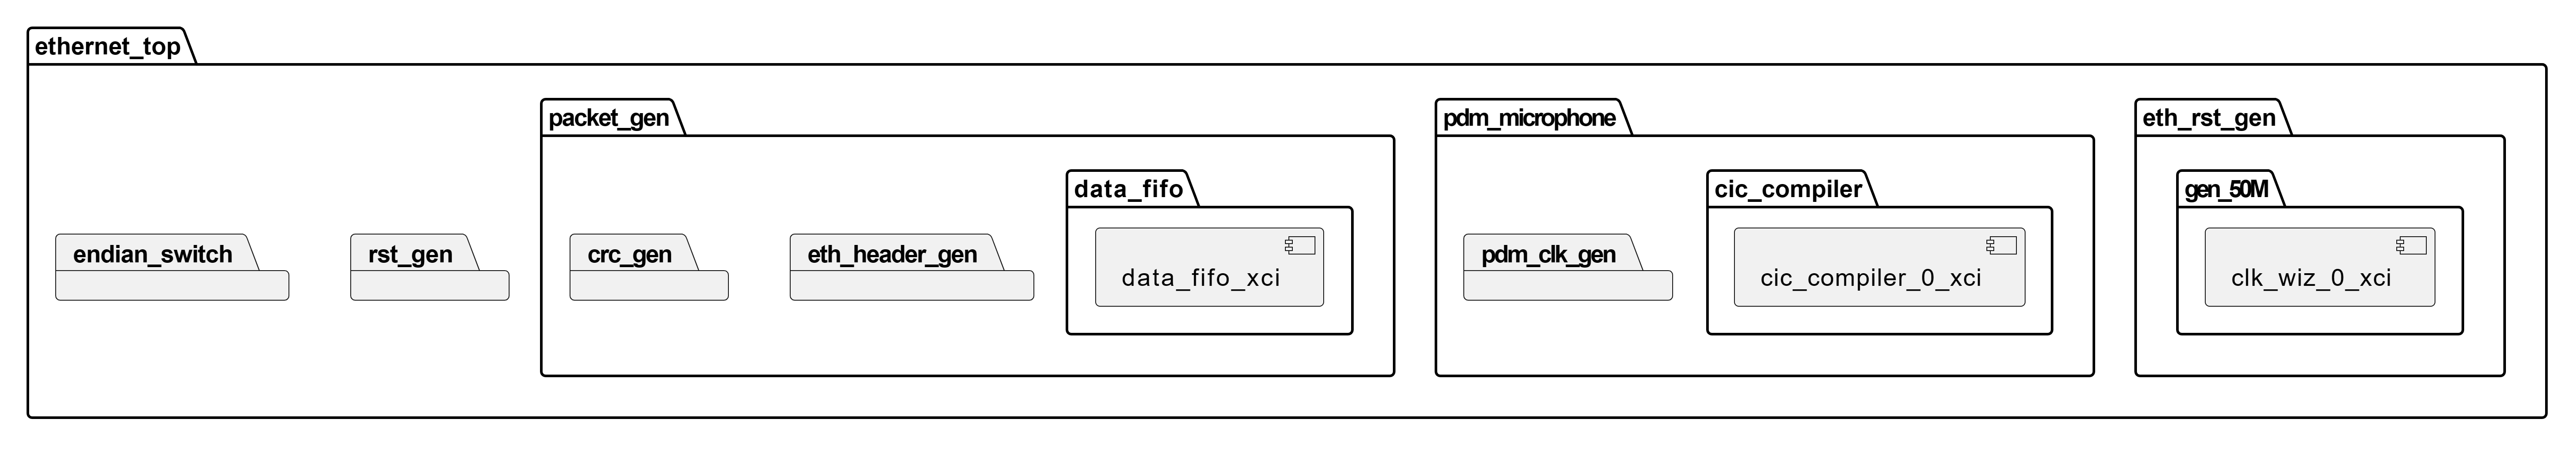
\includegraphics[width=1\linewidth]{Sections//IMPLEMENTATION//images/ModulePDM.png}
    \caption{PDM module architecture}
    \label{fig:pdm-mod-arch}
\end{figure}

\subsubsection{Microphone Digital Interface}
The FPGA directly interfaces with the microphone, which outputs the PDM signal. Our system is designed to handle the PDM signal in the following manner:

\begin{itemize}
    \item The PDM frequency, or the sampling frequency of the microphone, ranges between 1 MHz and 3.3 MHz. For our application, we have chosen 2.4 MHz, attainable through clock division since it is below the 5 MHz threshold.
    \item To address potential metastability issues arising from clock domain crossing, the design incorporates triple-registering.
    \item The PDM data undergoes processing by a Cascaded Integrator-Comb (CIC) filter. The configuration for the IP generation of the CIC filter is as follows (Refer Figure \ref{fig:cic-ip}):
    \begin{itemize}
        \item Five stages of integration and comb filtering.
        \item A decimation factor of 64, resulting in an effective sampling frequency ($F_s$) of 37.5 kHz, derived from the 2.4 MHz PDM signal.
    \end{itemize}
\end{itemize}

The FPGA is programmed to process the PDM data and convert it into Pulse Code Modulation (PCM) data, which is a standard format for audio signals.

\begin{figure}[htbp]
\centering
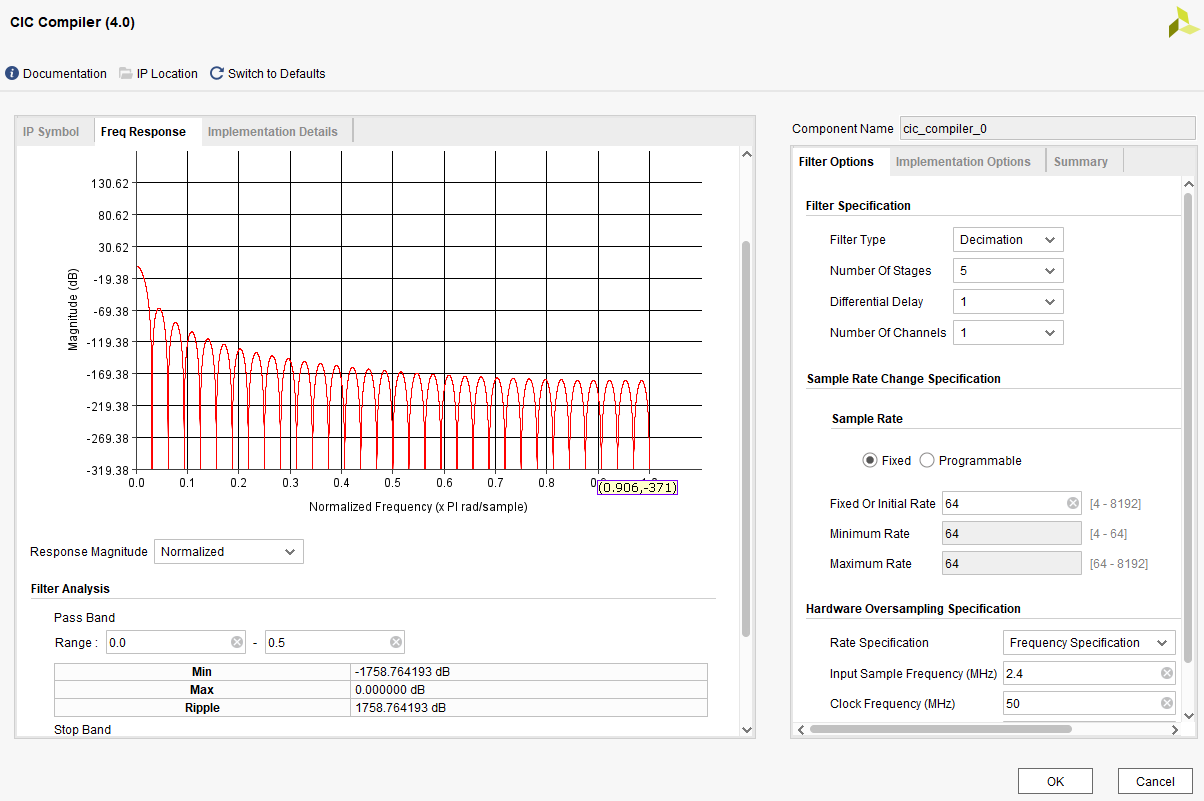
\includegraphics[width=.7\textwidth]{Sections/IMPLEMENTATION/images/cic-ip.png}
\caption{IP configurations of CIC compiler}
\label{fig:cic-ip}
\end{figure}


\subsubsection{Packet Processing on the Host Machine}

The process of handling Ethernet packets on the host machine is integral to the data analysis phase. The following methodology is adopted to capture and process the packets:

\begin{enumerate}
    \item Initialize a RAW\_SOCKET to intercept all Ethernet packets on the network interface.
    \item Implement packet filtering based on the MAC address to isolate the relevant data.
    \item Utilize a Python script for packet processing, which involves:
    \begin{itemize}
        \item Defragmenting the packet data sequences.
        \item Interpreting the payload as 32-bit big-endian integers.
        \item Normalizing the data by subtracting the mean (DC offset) and scaling the amplitude to fit within a -1 to +1 range.
        \item Converting the normalized data to 16-bit little-endian integers.
        \item Saving the final output as a .wav audio file.
    \end{itemize}
\end{enumerate}

An alternative approach entails the use of packet capture software, such as Wireshark, to acquire the packets. The collected packet data can subsequently be processed by a script that performs the operations mentioned earlier, thereby reconstructing the audio signal.


\subsection{Fast Fourier Transform of the PDM Audio Data}

The final part of the project demonstrates a practical example of signal processing on the audio data before transmitting it using the mechanism developed earlier. The Fast Fourier Transform (FFT) is an algorithm used to efficiently compute the Discrete Fourier Transform (DFT) and its inverse. The FFT exploits symmetries and recursive divide-and-conquer strategies to compute the Fourier transform in $O(N log N)$ time complexity, where N is the size of the input data
(refer to Figure \ref{fig:fft-mod-arch} for the implementation overview)

\begin{figure}
    \centering
    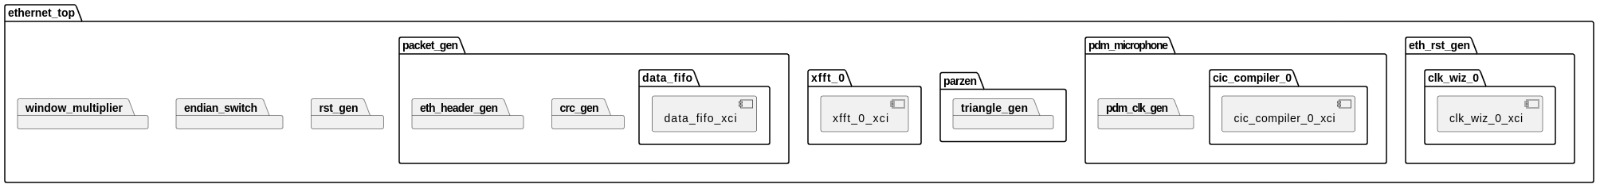
\includegraphics[width=1\linewidth]{Sections/IMPLEMENTATION/images/ModuleFFT.jpeg}
    \caption{FFT module architecture}
    \label{fig:fft-mod-arch}
\end{figure}


% This process involves the following steps before it is transmitted via ethernet:

\subsubsection{Windowing Operation using Parzen Window}
% When we use the FFT to measure the frequency component of a signal, we are basing the analysis on a finite set of data. The actual DFT algorithm assumes the finite data points are samples of a periodic signal over one time period. For the FFT, both the time domain and the frequency domain are circular topologies, so the two endpoints of the time waveform are interpreted as though they were connected together. When the measured signal is periodic and an integer number of periods fill the acquisition time interval, the FFT captures the frequency information accurately, as shown in Fig. 

% When the number of periods in the acquisition is not an integer, as in the case of real-time audio signals, the endpoints are discontinuous. These artificial discontinuities show up in the FFT as high-frequency components not present in the original signal. These frequencies can be much higher than the
% Nyquist frequency and are aliased between 0 and half the sampling rate. The spectrum obtained by using FFT, therefore, is not the actual spectrum of the original signal, but a smeared version. It appears as if the energy at one frequency leaks into other frequencies. This phenomenon is known as spectral leakage, which is depicted in Fig.

% The effects of performing FFT over a noninteger number of cycles can be minimized by using a technique called windowing. Windowing reduces the amplitude of the discontinuities at the boundaries of each finite sequence acquired by the digitizer. Windowing consists of multiplying the time record by a finite-length window with an amplitude that varies smoothly and gradually toward zero at the edges. This makes the endpoints of the waveform meet and, therefore, results in a continuous waveform without sharp transitions.
When employing the FFT for frequency analysis of signals within a finite dataset, it assumes periodicity in the time domain. The FFT treats both the time and frequency domains as circular, connecting the endpoints of the time waveform. In cases where the signal's period doesn't exactly fill the acquisition time, as in real-time audio, artificial discontinuities arise, causing spectral leakage. These spurious high-frequency components, appearing between 0 and half the sampling rate, are aliases of energy from other frequencies. To mitigate spectral leakage, windowing techniques are employed. Windowing involves multiplying the time record by a smooth, finite-length window, reducing discontinuity effects at the sequence boundaries and providing a more accurate representation of the signal's spectrum.

The Parzen Window is one such example of a windowing signal(\ref{fig:parzenwindow}). It is a fourth-order B-spline window, defined in the time domain as follows: 

\begin{figure}[htbp]
\centering
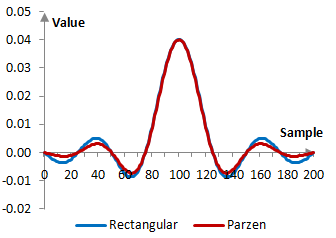
\includegraphics[width=.3\textwidth]{Sections/IMPLEMENTATION/images/parzenwindow-impulseresponse.png}
\caption{Impulse response of the Parzen window.}
\label{fig:parzenwindow}
\end{figure}

\begin{equation}
    w_0[n]=
    \begin{cases}
        1 - 6(\frac{N}{L/2})^2(1 - \frac{|n|}{L/2}) & \text{if } 0 \leq |n| \leq \frac{L}{4}\\
        2(1 - \frac{|n|}{L/2})^3 & \text{if } \frac{L}{4} \leq |n| \leq \frac{L}{2}
    \end{cases}
\end{equation}
\begin{equation}
    w[n]= w_0[n](n - \frac{N}{2}), 0 \leq n \leq N    
\end{equation}
Here, $L = N + 1$

\subsubsection{FFT on the windowed data}
We used the \texttt{x\_fft} IP available in the Xilinx Vivado IP-Catalog to perform a 256-point FFT on the audio data. The specifications of the IP are shown in Figure \ref{fig:fft-ip}

\begin{figure}[htbp]
\centering
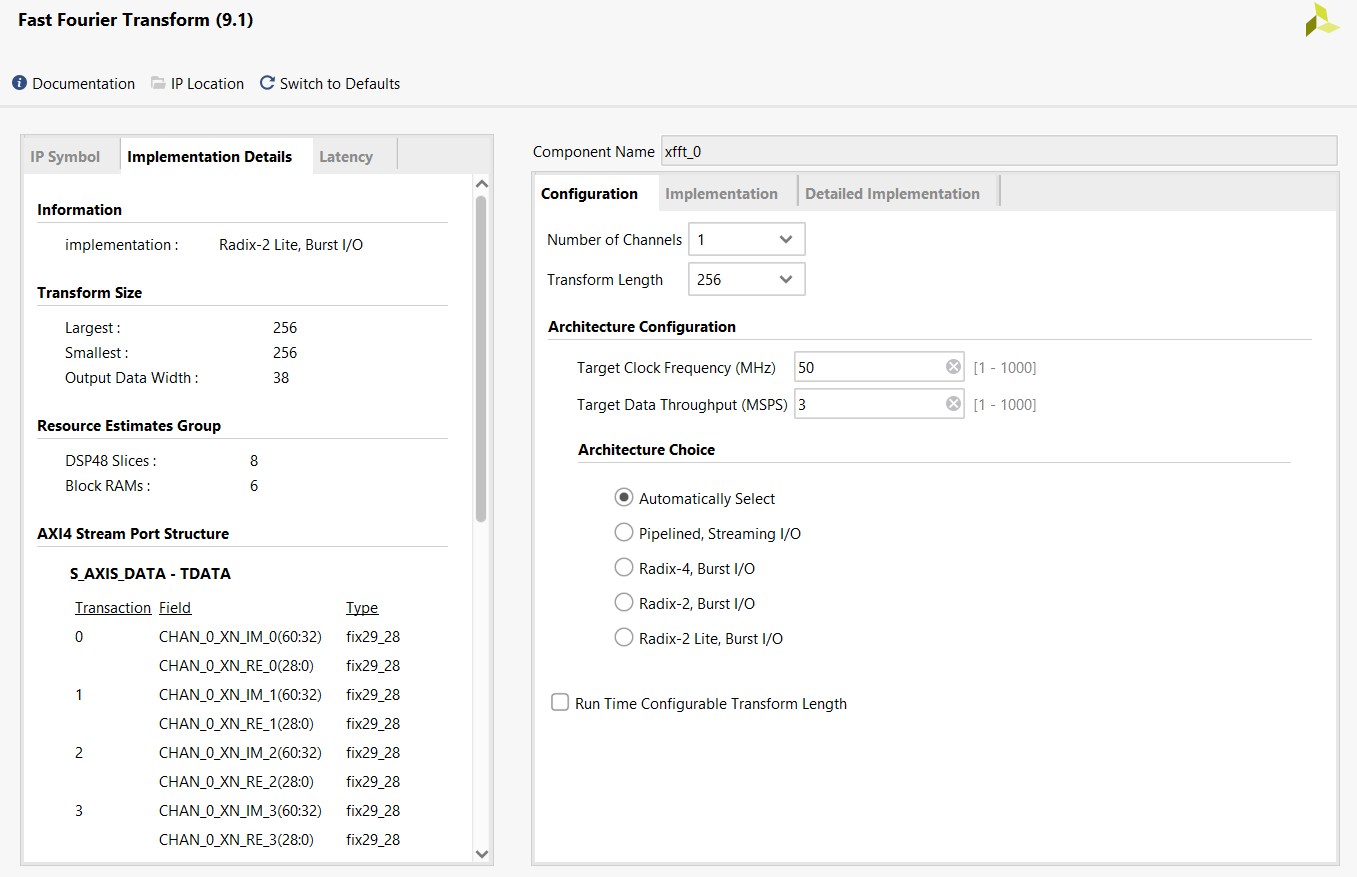
\includegraphics[width=.7\textwidth]{Sections/IMPLEMENTATION/images/fft-ip.png}
\caption{IP configurations of FFT}
\label{fig:fft-ip}
\end{figure}

% At the receiver's end, the following post-procesing steps are performed on the captured packets:

\subsubsection{Visualization of FFT at Receiver}
An empty \texttt{matplotlib} figure is initialised, with the x-axis ranging from 0 to 256 and the y-axis from 0 to 8. A function animate() is defined, which is called repeatedly to update the plot animation. Inside this function, the following operations are performed in a loop 16 times:
\begin{enumerate}
    \item Data packets are received from the RAW\_SOCKET.
    \item An \texttt{fftshift} operation is performed on the square root of the absolute value of the received data, to center the data about the origin.
    \item The computed values are updated to an accumulated average.
\end{enumerate}
 
The real-time plot displays a two-sided Fourier spectrum, which is symmetric about the origin. The functionality of the process is verified by testing the module on a single-frequency sine wave obtained from a tone generator.


